\section{Assignment 4}

\subsection{Implement the Kalman smoother and estimate the velocity and acceleration from noisy position measurements}

Starting with the same model described in assignment \ref{ass3}, the Kalman smoother is defined in two parts. a forward step consisting of standard Kalman filtering and a backward step in which the smoothing takes place.

In the forward step, a standard Kalman filtering procedure is carried out:
\begin{align*}
\hat x_{k+1\mid k+1}^f &= A\hat x_{k\mid k}^f +K_{k+1}(y_{k+1}-CA\hat x_{k\mid k}^f)\\
\hat x_{0\mid 0}^f&=\bar x_0\\
P_{0\mid 0}^f &= P_0\\
P_{k\mid k}^f &= P_{k-1\mid k-1}^f - KCP_{k-1\mid k-1}^f\\
P_{k+1\mid k}^f &= AP_{k\mid k}^fA^T + Q 
\end{align*}

Then in the backward step, smoothing is carried out as follows:
\begin{align*}
\hat x_{k\mid N}^s&=\hat x_{k\mid k}^f+\breve K_k(\hat x_{k+1\mid N}^s-\hat x_{k+1\mid k}^f)\\
\hat x_{N\mid N}^s&=\hat x_{N\mid N}^f
\end{align*}

where:
\begin{equation*}
\breve K_k = P_{k\mid k}^fA^T(P_{k+1\mid k}^f)
\end{equation*}

and the conditional covariance matrix $P_{k\mid N}$ satisfies:
\begin{align*}
P_{k\mid N}&=P_{k\mid k}^f+\breve K-k(P_{k+1\mid N}-P_{k+1\mid k}^f)\\
P_{N\mid N} &= P_{N\mid N}^fs
\end{align*}

The smoother is applied to a position signal with Gaussian noise and a signal with quantization noise, and compared to the estimation given by the Kalman filter. The results are shown in figures \ref{fig:kalman_s_gauss} and \ref{fig:kalman_s_quant}.


\begin{figure}[H]
\centering
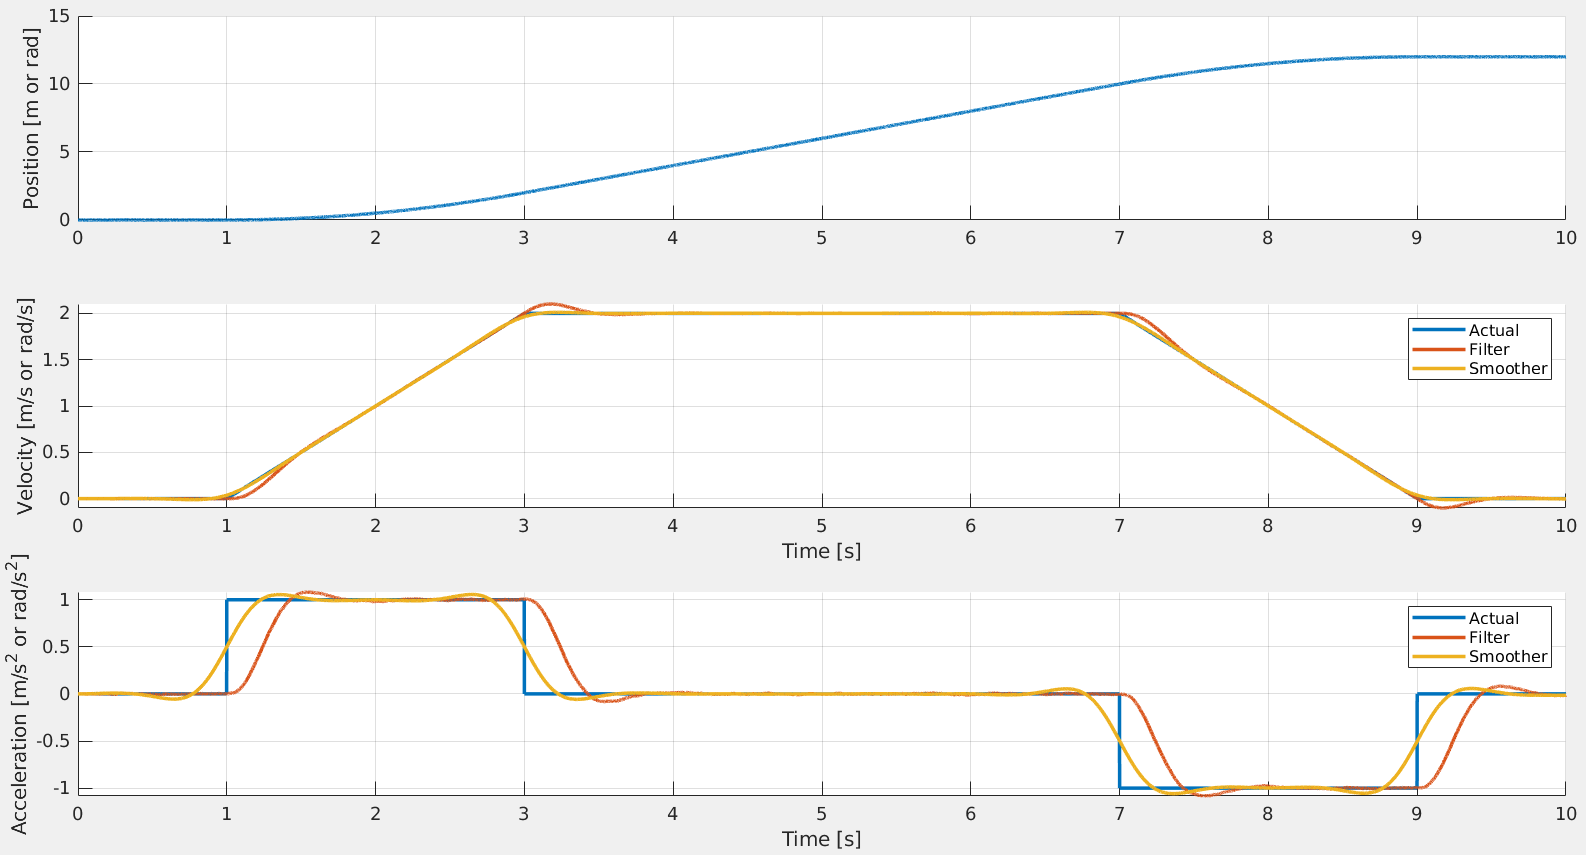
\includegraphics[keepaspectratio,width=\textwidth]{kalman_s_gauss}
\caption{Kalman smoother vs Kalman filter applied to a position signal with Gaussian noise}
\label{fig:kalman_s_gauss}
\end{figure}

\begin{figure}[H]
\centering
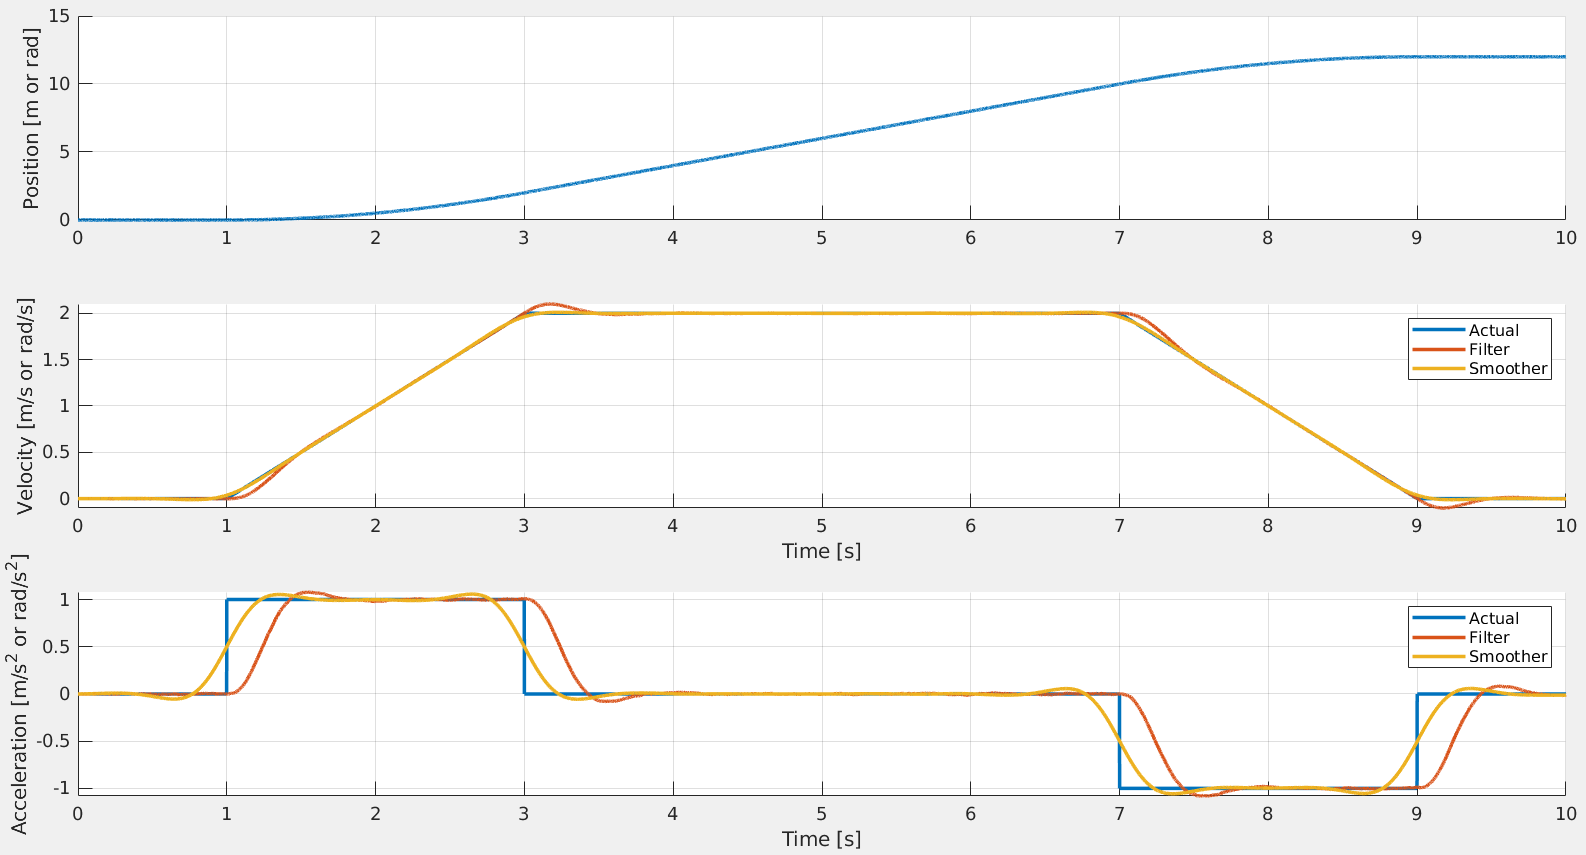
\includegraphics[keepaspectratio,width=\textwidth]{kalman_s_quant}
\caption{Kalman smoother vs Kalman filter applied to a position signal with quantization noise}
\label{fig:kalman_s_quant}
\end{figure}

The smoother effectively improves the estimation of the velocity, especially near the discontinuity points, and of the acceleration, making the shape of the estimation more closely match the "actual" acceleration.